\subsection{Feedback Configurations}
The main objective of the study was to evaluate two novel electrotactile feedback configurations' intuitiveness in providing proprioceptive information of a two DoF myoelectric prosthesis. 
The DoF's used were wrist rotation and closed hand, where each DoF was divided into four motion states, where a unique feedback was provided for the various states in each DoF. The electrode array used to deliver electrical stimulation can be seen in figure \ref{fig:pa:electrode}.
\begin{figure}[H]                 
	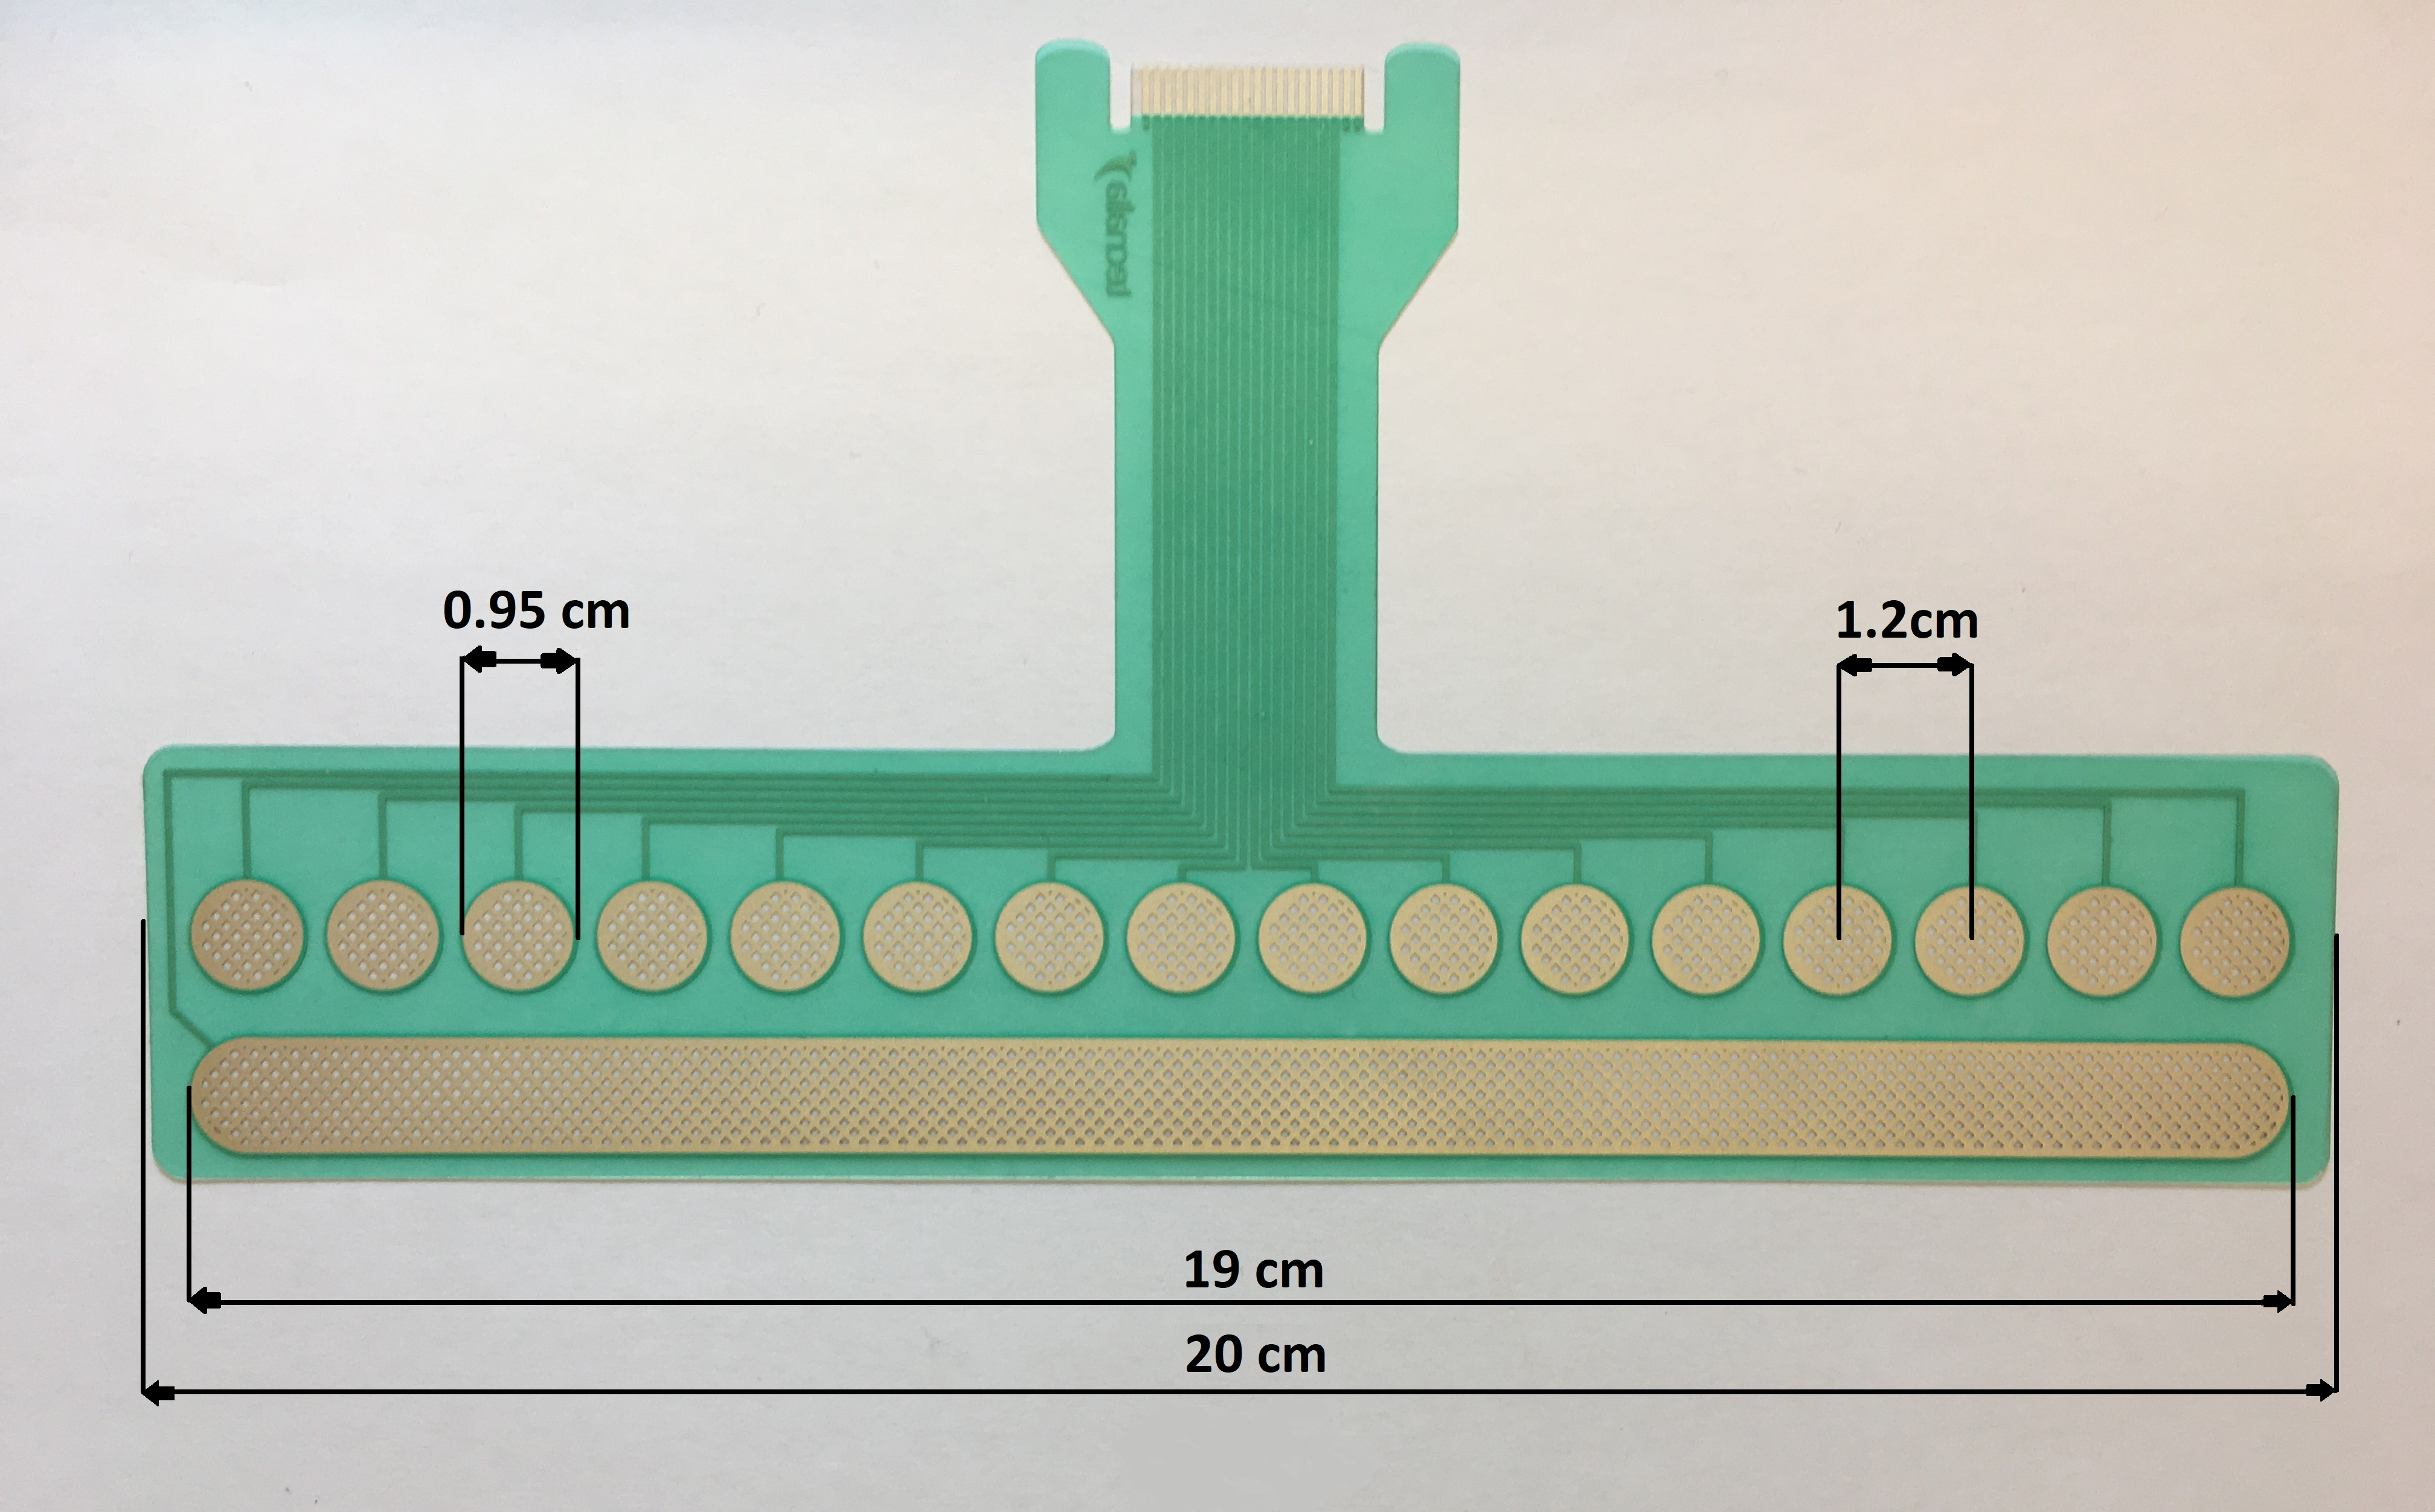
\includegraphics[width=.95\textwidth]{figures/electrode}  
	\caption{Image of the 16 multi-pad electrode array used for stimulation. It consisted of 16 circular cathode pads, which each shared a common anode.}
	\label{fig:pa:electrode} 
\end{figure}
The array electrode consisted of a single anode pad and 16 circular cathode pads of which the activation and current amplitude could be modulated individually. The pads comprised of conductive Ag/AgCl traces imprinted in a 150 $\mu m$ thick polyester layer. All pads were covered with conductive hydrogel (AG702, Axelgaard, Denmark) to enhance skin-electrode contact. The array electrode was placed around the contralateral lower arm of the dominant arm such that the end pads had a maximum gap of three cm centrally on the posterior side, when using a pronated arm as reference position. The following sections will present the two developed feedback configurations. 


\subsubsection{Spatial configuration}
The motivation behind the spatial configuration was to communicate wrist rotation by spatially rotate anteriorly placed active electrode pads and to communicate closed hand by narrowing the distance between posteriorly placed pads. 
This feedback design was chosen in order to intuitively mimic the directions of the motions in the included DoF's. An illustration of the spatial configuration can be seen in figure \ref{fig:pa:spatial}. 

\begin{figure}[h]                 
	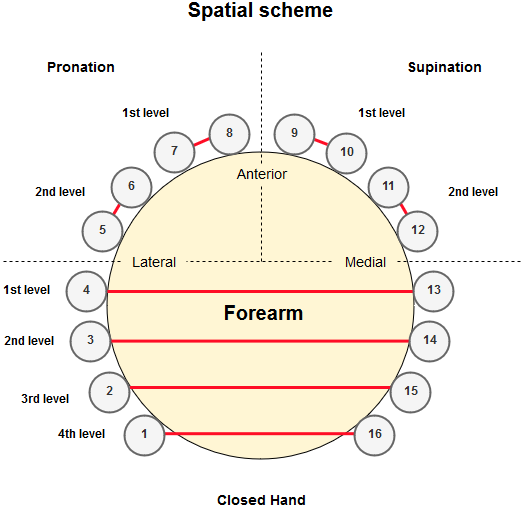
\includegraphics[width=.9\textwidth]{figures/El_array_spatial}  
	\caption{Transverse view of the developed spatial scheme fitted on the left arm of a subject. The levels written next to the pads pairs corresponded to the level of the prosthetic state; the higher the level, the higher the prosthetic state of the given movement was. When fitted on the right arm medial and lateral sides were reversed.}
	\label{fig:pa:spatial} 
\end{figure}
The pads were divided two groups each responsible for conveying information about a single DoF. The anteriorly placed pads were allocated for wrist rotation and the posteriorly placed for closed hand. The pads were furthermore paired such that each pair would represent one of four motion states in one DoF. For wrist rotation the pads were connected in side by side pairs. For right-handed subjects the activation of pads pairs would rotate laterally when increasing motion states during supination and rotate medially during pronation. The reversed activation was apparent for left-handed subjects. For the closed hand DoF the pairs consisted of oppositely located pads on the medial and lateral sides. When increasing motion states the active pairs would move posteriorly and the distance between active pads would become shorter. When the prosthesis was in a combined DoF state, the pads pairs corresponding to the level of the prosthetic state of each DoF would be active. Thus, a maximum of four pads could be active simultaneously. 

\subsubsection{Amplitude configuration}
The incentive behind the amplitude configuration was to convey information about the increase of prosthetic states by gaining the amplitude in electrode pad groups of four.
The areas of active pads allocated for the various motions was similar to the spatial configuration to intuitively resemble the prosthesis motions. An illustration of the amplitude configuration can be seen in figure \ref{fig:pa:amplitude}. The eight most anteriorly placed pads were used for wrist rotation and the four most posteriorly placed pads for closed hand. The eight pads used during wrist rotation were split such that the four most laterally placed were used during supination and four most medially placed were used during pronation for right-handed subjects. The pad activation was reversed for left-handed subjects. As the prosthetic state of a given movement would increase the the current amplitude in the pads corresponding to that movement would increase. When in combined DoF motion state, the pads corresponding to the level of the prosthetic state of each DoF would be active in the relative amplitude level. Thus, a maximum of eight pads could be active concurrently. The choice of groups of four electrode pads was decided upon to exploit the highest number of pads in the electrode array, while maintaining a symmetric distribution of possible active pads.

 \begin{figure}[h]                 
	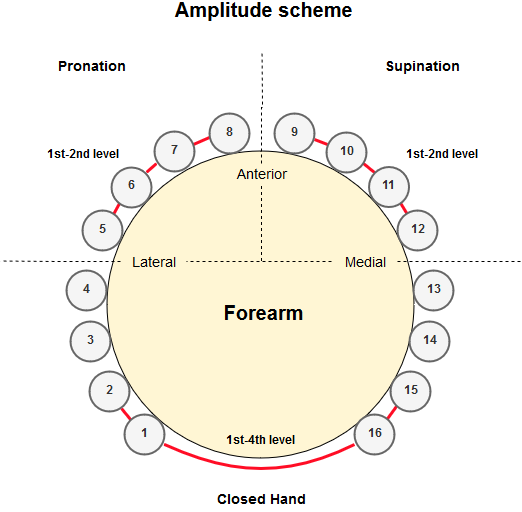
\includegraphics[width=.9\textwidth]{figures/El_array_amplitude}  
	\caption{Transverse view of the developed amplitude scheme fitted on the left arm of a subject. Different groups of four electrode pads were active during supination, pronation and closed hand, respectively. The amplitude of the active pads would increase with the increase of the prosthetic state; the higher the prosthetic state level the higher the current amplitude of the given pads.When fitted on the right arm medial and lateral sides were reversed.}
	\label{fig:pa:amplitude} 
\end{figure}


